\documentclass[german,a4paper]{llncs}

\usepackage[ngerman]{babel}
\usepackage{palatino}
\usepackage[latin1]{inputenc}
\usepackage{graphicx}
\usepackage[urlbordercolor={1 1 1}, citebordercolor={1 1 1}]{hyperref}
% Seitenr�nder
\usepackage{geometry}
\geometry{verbose,a4paper,tmargin=5.2cm,bmargin=5.2cm,lmargin=4.4cm,rmargin=4.4cm}

% Kopf- und Fusszeile
\usepackage{fancyhdr}
\pagestyle{fancy}
\renewcommand{\headrulewidth}{0pt}
\renewcommand{\footrulewidth}{0pt}
\fancyhead[EL]{\textsc{Florian Rapp}}																		% Hier bitte den/die Autor(en) angeben
\fancyhead[OR]{\textsc{Entwicklung der Open-Street-Applikation f�r Windows Phone 7}}																				% Hier bitte den Dokumententitel angeben
\fancyfoot[EC,OC]{}
\begin{document}


\title{Entwicklung der Open-Street-Applikation f�r Windows Phone 7}
\author{Florian Rapp}
\institute{Universit�t Ulm, Abt. DBIS\\
\email{florian.rapp@uni-ulm.de}}
\maketitle

\begin{abstract}
Diese Arbeit besch�ftigt sich mit der Entwicklung einer Routing- und Navigationsapplikation, namentlich der \textit{Open Street App}, f�r das mobile Betriebssystem Windows Phone 7 (\textit{WP7}). Es wird aufgezeigt welche Schritte von der Idee dieser Applikation bis zur Fertigstellung umgesetzt, und welche Probleme und Herausforderungen �berwunden werden mussten. Die Arbeit soll einen grundlegenden Eindruck der pratischen Entwicklung f�r WP7 vermitteln.
\end{abstract}

\section{Einleitung}
\subsection{Rahmen der Arbeit}
Im Herbst 2010 ver�ffentlichte die Firma Microsoft ihr eigenes Betriebssystem f�r Smartphones, Windows Phone 7 (\textit{WP7}). Basierend auf WinCE 7, allerdings mit einem komplett neuen und modernen User Interface, sollte ein flexibles, innovatives System auf den Markt gebracht werden. Um mit den Branchenf�hrern \textit{Apple iOS} und \textit{Android} konkurrieren zu k�nnen, wurde insbesondere die einfache und schnelle Entwicklung von Applikationen f�r das neue System von Microsoft angepriesen. Im Rahmen des Seminars \textit{Entwicklung f�r Windows Phone 7} der Abteilung \textit{Datenbank- und Informationssysteme} der Universit�t Ulm, war es unser Ziel zu pr�fen wie effektiv sich Programme f�r WP7 zum aktuellen Stand entwickeln lassen.
\subsection{Idee der Open Street App}
Im Blickpunkt unserer Entwicklung stand nicht nur das reine Erstellen einer Applikation, sondern gerade auch die Verwendung der von Microsoft bereitgestellten Controls und Bibliotheken. Wir wollten herausfinden ob diese sich effektiv und schnell integrieren lassen. Zum Zeitpunkt des Seminarbeginns war f�r WP7 keine zufriedenstellendes Third-Party-Routing verf�gbar. WP7 liefert von sich aus eine Karte/Routing-Applikation. Unsere Idee war es nun eine eigene Software zu schreiben, welche den Anforderungen der mitgelieferten \textit{Karten-App} gen�gt und falls m�glich �bertrifft, unter Verwendung der erw�hnten Controls.
\subsection{Aufbau dieser Arbeit}
Im zweiten Kapitel wird erkl�rt mit welchen Quellen und Umsetzungsmitteln gearbeitet wurde um Kartendaten und zugeh�rige Informationen zu erlangen und darzustellen. Das folgende Kapitel besch�ftigt sich mit der Gestaltung der Applikation im WP7 typischen UI-Stil. Hierbei wurde besonderes Augenmerk gelegt auf ein konsistentes Look-and-Feel im Vergleich zu den native Applikationen f�r WP7. Kapitel vier berichtet exemplarisch von den Herausforderungen und Problemen die bei der Entwicklung aufgekommen sind. Kapitel f�nf erkl�rt wie einmal entwickelte Applikationen ihren Weg auf den Markt finden. Hier wird auf den Marketplace und die Zukunft der Open Street App eingegangen. Im letzten Kapitel wollen wir einen Ausblick �ber die m�glichen Entwicklungen von WP7 geben sowie ein Fazit zu der Entwicklung in diesem fr�hen Stadium ziehen.\cite{cloud} \cite{coding} \cite{launch} \cite{silverlight} \cite{apps} \cite{osm} \cite{yahoo} \cite{bing}

\section{Open Street Map und Konsorten}

\subsection{Umsetzung des Map-Controls}
\subsection{Verwendung von Services}

\section{Umsetzen der WP7 Designkonzepte}
\subsection{WP7 Look and Feel}

\section{Herausforderungen}
\subsection{Probleme der gegebenen Controls}
\subsection{Routing}
Text zu Routing
\begin{center}
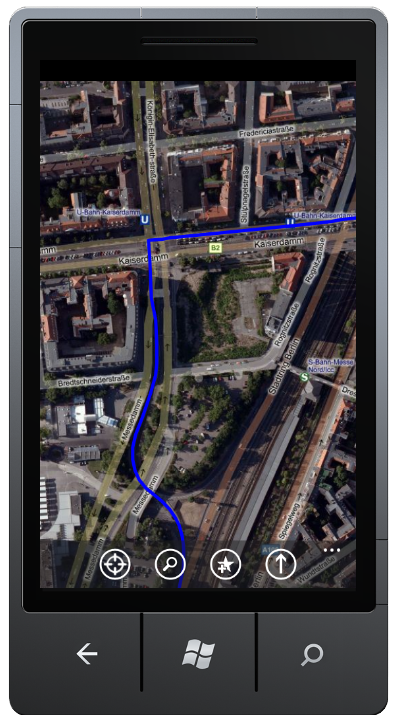
\includegraphics[width=5.0cm,height=10.0cm]{images/route.png}
\end{center}
\begin{figure}
\caption{Vereinfachte Route}
\end{figure}

\section{Marketplace}
\subsection{Struktur}
\subsection{Entwicklung}
\subsection{Zukunft der Open Street App}
�berlegung ob kostenpflichtig oder nicht. Werbung. Ver�ffentlichung im April 2011. Wirklich.

\section{Ausblick und Fazit}
\subsection{Weiterentwicklung der Plattform}
\subsection{Chancen f�r die Zukunft}
\subsection{Fazit}
Entwickeln toll. Schnelle Ergebnisse.

\bibliography{wp7seminar}
\bibliographystyle{plain}

\end{document}
